\newcommand{\eksp}{eksponencijalne funkcije}
    Eksponencijalna funkcija je funkcija oblika:
    \[f(x) = a^x,\;a > 0,\; a \neq 1\]
    \noindent Derivacija eksponencijalne funkcije je esksponencijalna funkcija.

\subsubsection{Domena i kodomena \eksp}
    Domena eksponencijalne funkcija je skup \(\mathbb{R}\).
    Kodomena eksponencijalne funkcije je skup \(\mathbb{R^+}\) jer je pozitivan realni broj na neku potenciju je pozitivan realni broj.

\subsubsection{Graf \eksp}
    Specifičnost grafa eksponencijalne funkcije je da uvijek prolazi kroz točku \((0, 1)\).
    Mijenjamo li bazu \(a\), mijenja se \emph{brzina} rasta. Dodavanjem slobodnog koeficijnta mjenjanmo odsječak na y-osi.
    \begin{figure}[ht]
        \centering
        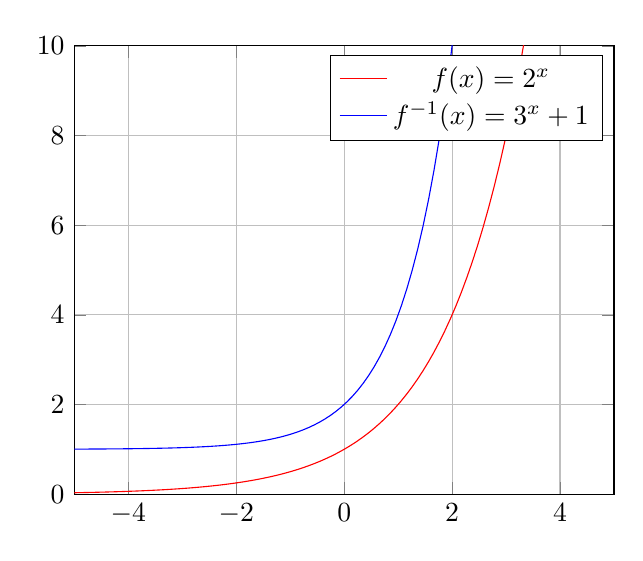
\begin{tikzpicture}
            \begin{axis}[
                grid=major,
                ymin=0,
                ymax=10,
                xmin=-5,
                xmax=5,
            ]
                \addplot[
                    color = red,
                    samples = 100
                ]{2^x};
                \addlegendentry{\(f(x) = 2^x\)}
                \addplot[
                    color = blue,
                    samples = 100
                ]{3^x + 1};
                \addlegendentry{\(f^{-1}(x) = 3^x + 1\)}
            \end{axis}
        \end{tikzpicture}
        \caption{Grafovi eksponencijalne funkcije s različitim parametrima}
        \label{fig:template}
    \end{figure}

\subsubsection{Nultočke i točke u kojima graf sječe y-os \eksp}
    Eksponencijalna funkcija nema nultočke.
    Eksponencijalna funkcija uvijek sječe y-os u točki \((0, 1)\):
    \[f(0) = a^0 = 1\]

\subsubsection{Parnost i neparnost \eksp}
    Funkcija nije ni parna ni neparna jer ne zadovoljava definicije u \ref{par}.

\subsubsection{Periodičnost \eksp}
    Funkcija nije periodična.

\subsubsection{Monotonost \eksp}
    Funkcija je strogo rastuća.

\subsubsection{Omeđenost \eksp}
    Funkcija nije omeđena.

\subsubsection{Injektivnost i surjektivnost \eksp}
    Eksponencijalna funkcija je bijekcija. Injekcija je jer vrijedi:
    \begin{equation*}
        \begin{split}
            f(x_1)      &= f(x_2) \\
            a^{x_1}     &= a^{x_2} \\
            x_1         &= x_2
        \end{split}
    \end{equation*}
    Surjektivna je po definiciju, dakle bijekcija je.

\subsubsection{Inverz \eksp}
    Inverz logaritamske funkcije je eksponencijalna funkcija.
    \begin{figure}[ht]
        \centering
        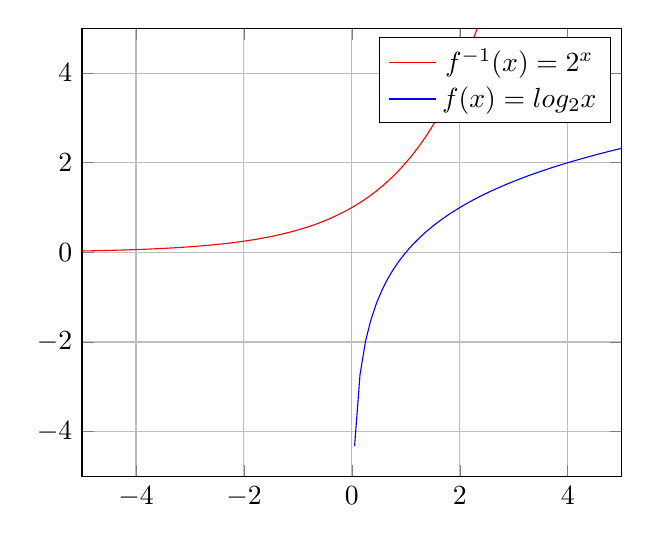
\begin{tikzpicture}
            \begin{axis}[
                grid=major,
                ymin=-5,
                ymax=5,
                xmin=-5,
                xmax=5,
            ]
                \addplot[
                    color = red,
                    samples = 100
                ]{2^x};
                \addlegendentry{\(f^{-1}(x) = 2^x\)}
                \addplot[
                    color = blue,
                    samples = 100
                ]{log2(x)};
                \addlegendentry{\(f(x) = log_2x\)}
            \end{axis}
        \end{tikzpicture}
        \caption{Grafovi funkcije i njenzinog inverzna}
        \label{fig:template}
    \end{figure}
    \\